\section{Autoencoders}
Autoencoders are a subset of neural networks. Whereas a general neural network
 in principle can take any shape, autoencoders are more restrictive.
This restrictiveness can in its most general sence we condensed 
into the following points:
\begin{itemize}
    \item Same number of output categories as input categories  
    \item A latent space with smaller dimensionality than the input/output layer  
\end{itemize}
What we end up with are two funnel shaped parts linked together. The two funnels are 
called the encoder (left funnel) and decoder (right funnel) respectively. This architecture is not 
accidental, but rather designed with a very specific solution of ploblems in mind, reconstruction. 
A good example to illustrate this is image reconstruction, illustrated in figure \ref{fig:ae_denoise}. 
Suppose you have an image, and want to reconstruct it. By feeding the encoder an image, 
and comparing the decoder output to the actual image, the autoencoder can tune itself to recreate the images it trains on. 

\begin{figure}[h!]
    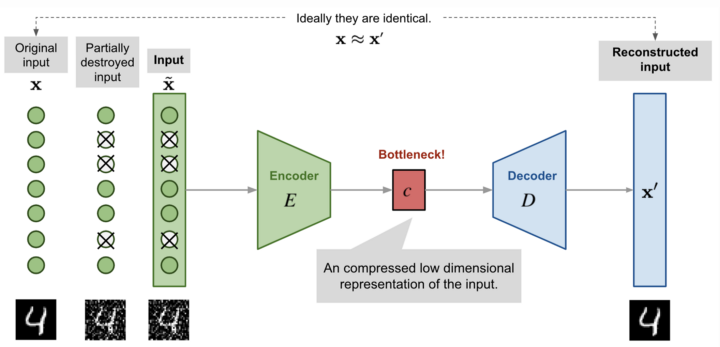
\includegraphics[width=\linewidth]{Figures/Machinelearning/autoencoder_imagedenoising.png}
    \caption[Conceptual autoencoder]{Figure depicting a model for an autoencoder. Here the input $\bf{x}$ is the original image, $\bf{x'}$ is a reconstructed version of $\bf{x}$, $g_{\phi}$ is the encoder, $f_{\theta}$ is the decoder, and $z$ is the latent space. Found 14.01.23 \href{https://lilianweng.github.io/posts/2018-08-12-vae/autoencoder-architecture.png}{here} \cite{weng2018VAE}. }
    \label{fig:ae_denoise}
\end{figure}

Mathematically this is is represented as follows\cite{weng2018VAE}. Using the annotations of each component in figure \ref{fig:ae_denoise} the decoded information is defined as follows 
\begin{equation*}
    \bf{z} = g_{\phi}(\bf{x}),
\end{equation*}    
and the reconstruction given as 

\begin{equation*}
    \bf{x'} = f_{\theta}(g_{\phi}(\bf{x})).
\end{equation*}  

The parameters $(\phi,\theta)$ are the tuneable parameters adjusted according to the loss function. In our case, the goal is
reconstruction without copying, thus we can simply use mean squared error, given as 

\begin{equation}\label{eq:loss_ae}
    L_{AE} (\phi,\theta) = \frac{1}{N}\sum_{i=0}^{N-1} \left(\bf{x}^{i} - f_{\theta}(g_{\phi}(\bf{x}^{i}))\right)^{2}.
\end{equation}

\section{Variational autoencoders}
Another popular method for reconstruction is the so called variational autoencoder. The work by Kingman and Welling \cite{VAE} showed how
one can use the variational bayesian approach for efficient approximate posterior inference, leading to the use of variational autoencoders.
Here, contrary to regular autoencoders, the latent space is thought of as a distribution. In the context of reconstruction, this means that
we want to create a latent space distribution based on the true distribution in the data, and use this latent space distribution to then generate
data given that latent space. 
\subsection*{Variational Bayes}
Let's assume some dataset $X = \{x^{(i)}\}_{i=1}^{N}$ with N samples for a variable x, and also assume that the generation of the data comes from 
some random variable z. We also assume that this variable z is generated from a prior distribution $p_{\theta}(z)$ and that the data is then 
generated from a conditional distribution $p_{\theta}(x|z)$, and that both their respective probability density functions are sufficiently 
differentiable with respect to parameters $\theta$ and z. We then have that the true posterior distribution is given by 
$p_{\theta}(z|x) = p_{\theta}(z)p_{\theta}(x|z)/p_{\theta}(x)$. The work done by Kingman and Welling \cite{VAE} was motivated by the fact that
$p_{\theta}(z|x)$ more often than not is intractable\footnote{Intractability here refers to the inability to evaluate or differentiate 
a given distribution or function, or difficulty with solving a problem due to a large parameter space or finding the global optimum of 
a complex function. }, thus instead we will try to approximate the true posterior with a variational approximation $p_{\theta}(z|x) \approx q_{\phi}(z|x)$.   
It can from here on out be useful to think of $q_{\phi}(z|x)$ as a probabilistic encoder, as it for a given data point x will produce a distribution
over possible values for z, the latent space, that the datapoint could have been generated from. Similarly, is can be useful to think of the   
$p_{\theta}(z|x)$ as a probabilistic decoder, as it for a given z will produce a distribution over possible values for x.

\subsubsection*{The variational bound}
It can be shown that the marginal likelyhood can be written as follows:
\begin{equation}
    log\, p_{\theta}(x^{(i)}) = D_{KL}(q_{\phi}(z|x^{(i)})||p_{\theta}(z|x^{(i)})) + \mathcal{L}(\theta, \phi;x^{(i)}),
\end{equation}

where the first term on the right hand side is the Kullback-Leibler (KL) diverge\footnote{The KL divergence is a measure of how one 
probability distribution is different from a second, reference probability distribution. It is often used as a distance measure 
between two probability distributions.} and the second term is the evidence lower bound (ELBO) on the marginal likelyhood. As the KL divergence
is non-negative, the ELBO will always be equal to or less than the marginal likelihood, written below:
\begin{equation}\label{eq:elbo_leq1}
    log\, p_{\theta}(x^{(i)}) \geq \mathcal{L}(\theta, \phi;x^{(i)}) = \mathbb{E}_{q_{\phi}(z|x)}[-log\, q_{\phi}(x|z)+log\, p_{\theta}(x|z)].
\end{equation}
Rewriting we get that the ELBO is given as:
\begin{equation}\label{eq:elbo_leq2}
    \mathcal{L}(\theta, \phi;x^{(i)}) =  - D_{KL}(q_{\phi}(z|x^{(i)})||p_{\theta}(z|x^{(i)})) + \mathbb{E}_{q_{\phi}(z|x^{(i)})}[log\, p_{\theta}(x^{(i)}|z)],
\end{equation}
which is also known as the loss function for variational inference. As a loss function, this needs to be differentiated with respect to 
$(\phi, \theta)$, but as shown by Kingman and Welling \cite{VAE}, the common method using Monte Carlo gradient estimator have high variance,
and thus is not ideal. 

\subsubsection*{The Stochastic gradient variational bayes (SGVB) estimator}
Kingman and Welling \cite{VAE} instead proposes a practical estimator that both deals with effectivity with large datasets, aswell as the 
issue of intractability. This estimator is called the stochastic gradient variational bayes (SGVB) estimator, and first assumes an approximate 
posterior $q_{\phi}(z|x)$. Under certain conditions, as shown in subsection \ref{sec:reparameterization}, we can reparameterize this approximate
posterior to a random variable $\tilde{z} \thicksim q_{\theta}(z|x)$, by doing a differentiable transformation $g_{\phi}(\epsilon|x)$, such that 
\begin{equation*}
    \tilde{z} = g_{\phi}(\epsilon|x), \quad \epsilon \thicksim p(\epsilon),
\end{equation*}
where $\epsilon$ is a noise variable.\par 
Using Monte Carlo estimates of expectations of a function $f(z)$ with respect to $q_{\theta}(z|x)$, Kingman and Welling \cite{VAE} shows that:
\begin{equation}
    \mathbb{E}_{q_{\theta}(z|x^{(i)})}[f(z)] = \mathbb{E}_{p(\epsilon)}[f(g_{\phi}(\epsilon, x^{(i)}))] \approx \frac{1}{L}\sum_{l=1}^{L}f(f(g_{\phi}(\epsilon^{(l)}, x^{(i)}))),
\end{equation}
where $\epsilon^{(l)} \thicksim p(\epsilon)$. Using this technique, and assuming that the KL divergence 
$D_{KL}(q_{\phi}(z|x^{(i)})||p_{\theta}(z|x^{(i)}))$ can be integrated analytically, we only get one term in 
equation \ref{eq:elbo_leq2} that requires estimation by sampling: $\mathbb{E}_{q_{\phi}(z|x^{(i)})}[log\, p_{\theta}(x^{(i)}|z)]$. 
What we end up with is a version of the SGVB estimator: $\tilde{\mathcal{L}}^{B}(\theta, \phi; x^{(i)}) \backsimeq 
\mathcal{L}(\theta, \phi; x^{(i)})$. This is given as:

\begin{equation}
    \mathcal{L}(\theta, \phi; x^{(i)}) = -D_{KL}(q_{\phi}(z|x^{(i)})||p_{\theta}(z)) + \frac{1}{L}\sum_{l=1}^{L} (\log p_{\theta}(x^{(i)}|z^{(i,l)})),
\end{equation}
where $z^{(i,l)} = g_{\phi}(\epsilon^{(i,l)}, x^{(i)})$ and $\epsilon^{(i)} \thicksim p(\epsilon)$. What we now have is a loss function that contains two terms. 
The first term, the KL divergence, acts as a regularizer, whereas the other term acts as a negative reconstruction error. In fact, we have here two objectives, 
we want to minimize the ELBO, $\mathcal{L}(\theta, \phi; x^{(i)})$, by minimizing the KL divergence and maximizing the expected log-likelihood. 

\subsubsection*{Reparameterization}\label{sec:reparameterization}
If the latent space is assumed to be a continous variable sampled from a conditional continous distribution 
$z \thicksim q_{\phi}(z|x)$, then we can reparametrize z as a deterministic variable. This is very useful as 
we then can rewrite the expectation of the conditional distribution such that the Monte Carlo estimate of 
the expectation is differentiable with respect to the parameters $\phi$. The proof can be found in the article\cite{VAE}.  
Now let's take the example of the univariate Gaussian distribution. First, let $z \thicksim p(z|x) = \mathcal{N}(\mu, \sigma^2)$. 
Then, a reparametrization of z can be $z = \mu + \sigma\epsilon$, where $\epsilon \thicksim \mathcal{N}(0,1)$. 
Thus 

\begin{equation*}
    \mathbb{E}_{\mathcal{N}(z; \mu, \sigma^2)}[f(z)] \backsimeq  \frac{1}{L}\sum_{l=1}^L f(\mu + \sigma\epsilon^{(l)}).
\end{equation*}

\subsection*{Variational autoencoders}
Now, this variational bayes can then be used to create a variational autoencoder. This contains two neural networks, the generative model $p_{\theta}(x|z)$,
as well as the probabilistic encoder $q_{\phi}(z|x)$, which is used to approximate the posterior $p_{\theta}(z|x)$. We now let the prior over 
the latent space be a multivariate Gaussian, lacking parameters: $p_{\theta}(z) = \mathcal{N}(z;0,I)$. We also have that $p_{\theta}(x|z)$ is a multivariate Gaussian,
with a distribution generated from z, whilst $p_{\theta}(z|x)$ is in fact intractable. If we now assume that the true (intractable) posterior 
is a Gaussian with approximately diagonal covariance, we can let the variational approximate posterior be a multivatiate Gaussian:
\begin{equation}
    log\, q_{\theta}(z|x^{(i)}) = log\, \mathcal{N}(z;\mu^{(i)},\sigma^{2(i)}I),
\end{equation}
where the mean and standard deviation are given by the neural network. Now, we sample from the approximate posterior $z^{(i,l)} \thicksim q_{\theta}(z|x^{(i)})$
where $z^{(i,l)} = g_{\phi}(x^{(i)}, \epsilon^{(l)}) = \mu^{(i)} + \sigma^{(i)} \odot \epsilon^{(l)}$, $\epsilon^{(l)} \thicksim \mathcal(N)(0,I)$ and $\odot$
is the elementwise product. If both the prior $p_{\theta}(z)$ and $q_{\theta}(z|x)$ are Gaussian, the KL divergence can be computed analytically, and it 
can then be showed\cite{VAE} that the variational approximate posterior is:

\begin{equation}\label{eq:loss_vae}
    \mathcal{L}(\theta, \phi;x^{(i)}) \simeq \frac{1}{2}\sum_{j=1}^{J}(1 + log\, ((\sigma^{(i)}_{j})^2) - (\mu^{(i)}_{j})^2 - (\sigma^{(i)}_{j})^2) +\frac{1}{L}\sum_{l=1}^{L}log\, p_{\theta}(x^{(i)}|z^{(i,l)}),
\end{equation}

where $z^{(i,l)} = \mu^{(i)} + \sigma^{(i)} \odot \epsilon^{(l)}$ and $ \epsilon^{(l)} \thicksim \mathcal{N}(0,I)$. 




\begin{figure}[h!]
    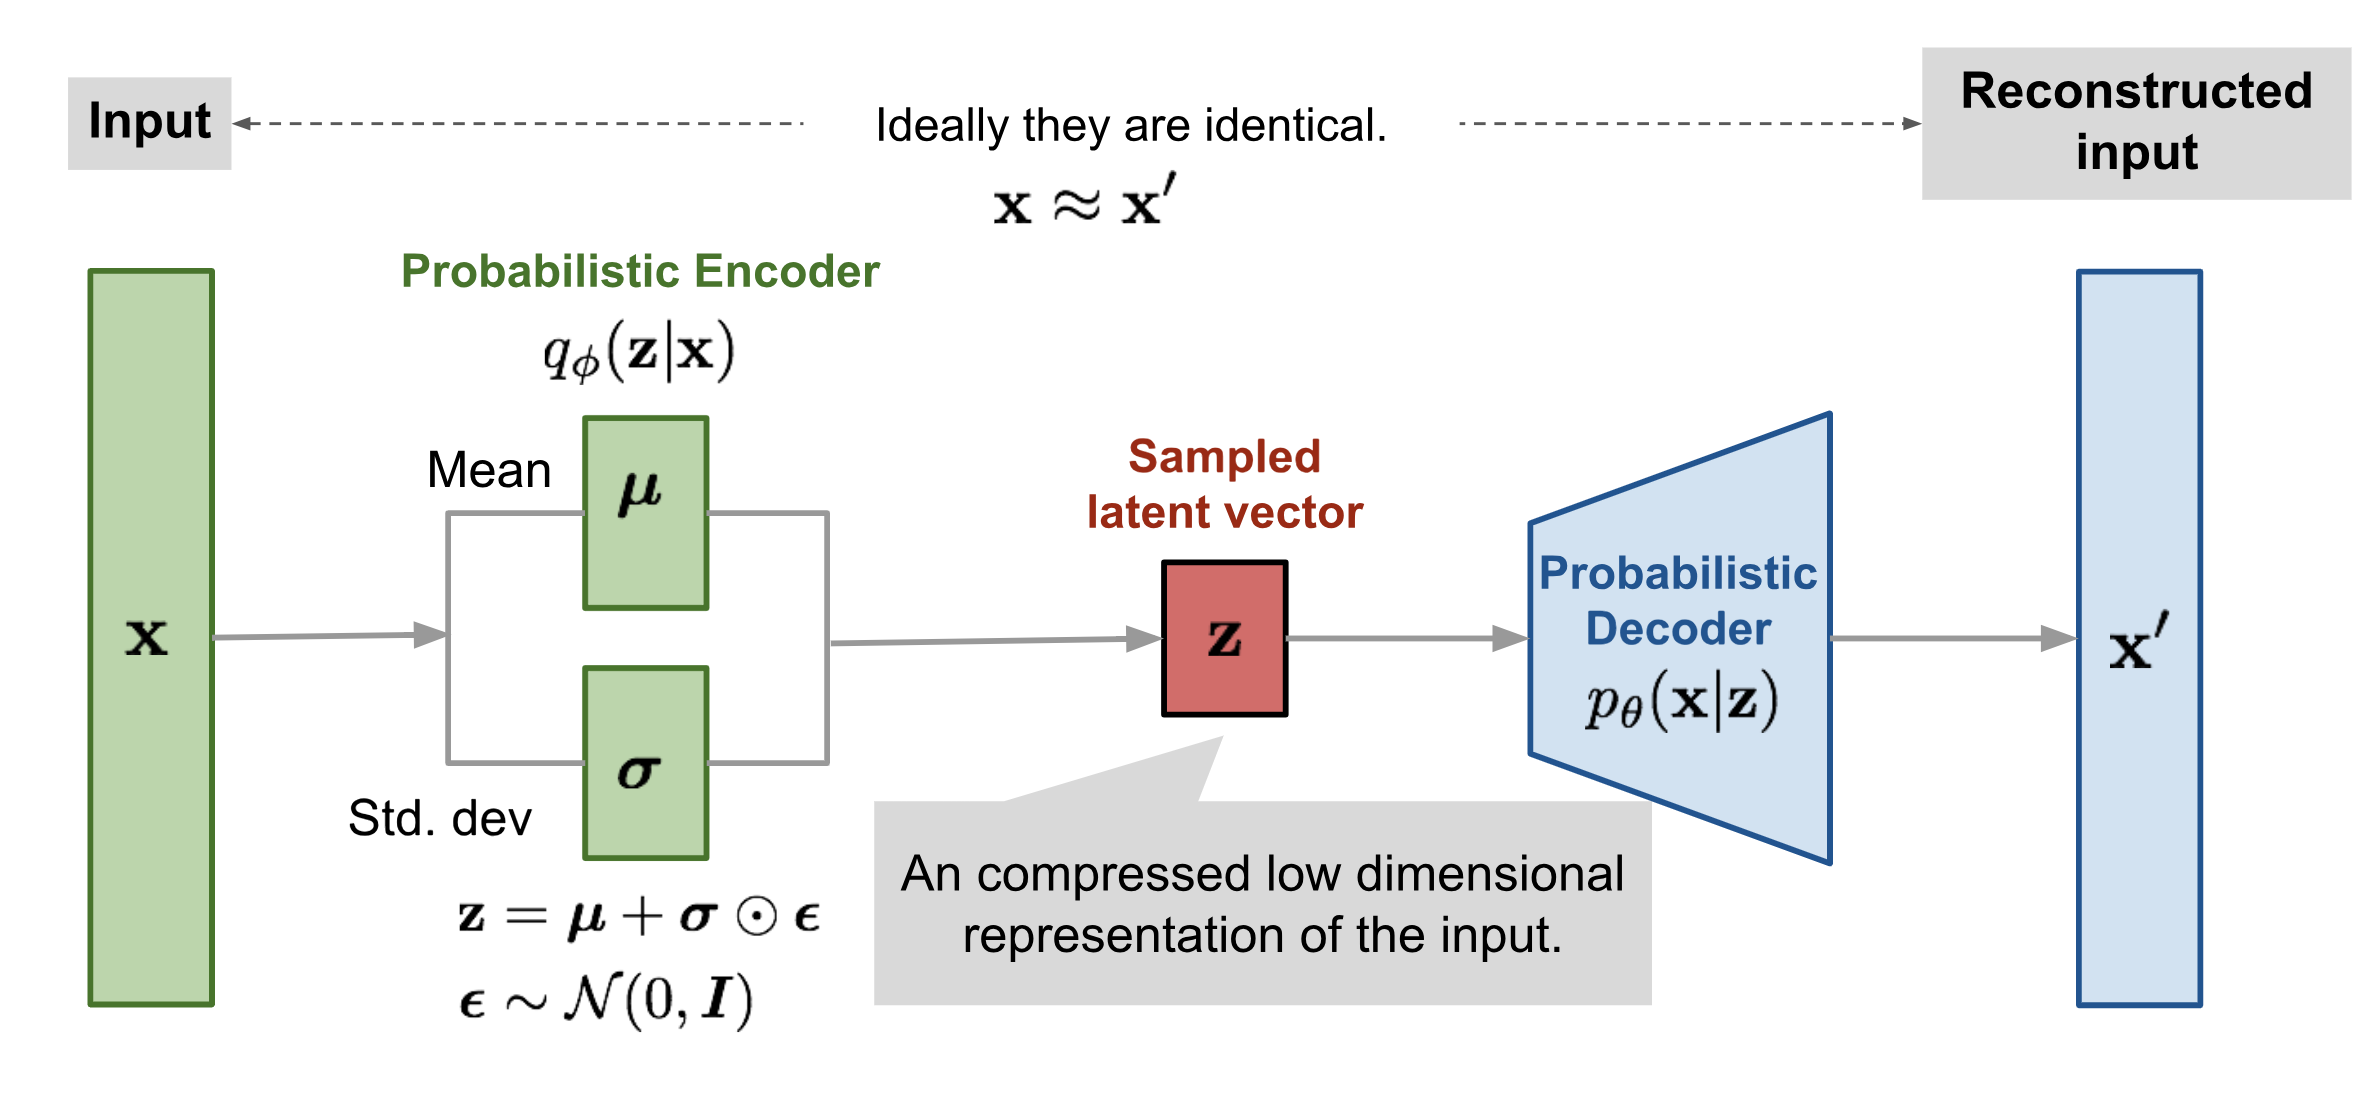
\includegraphics[width=\linewidth]{Figures/Machinelearning/vae-gaussian.png}
    \caption{Figure depicting a model for a variational autoencoder. Found 14.01.23 \href{https://lilianweng.github.io/posts/2018-08-12-vae/vae-gaussian.png}{here} \cite{weng2018VAE}. }
    \label{fig:vae}
\end{figure}

Figure \ref{fig:vae} is a graphical representation of the variational autoencoder. The encoder is a neural network, which takes 
the input $\bf{x}$ and maps the input to a latent space by creating a Gaussian distribution. The decoder is a neural network, 
which takes the latent space $\bf{z}$ and outputs the parameters of a Gaussian distribution for the data.
The loss function is given by equation \ref{eq:loss_vae}.